\mychapter{Introdução}
\label{Cap:introducao}

É observável uma crescente necessidade de se obter confiabilidade, flexibilidade e economia em um ambiente industrial. Devido a essas necessidades, a automação e elementos de redes industriais devem estar inseridos em qualquer planta industrial \cite{salazar2006instrumentaccao}. 

Um modelo hierárquico definido pela IEC 62264 representa de forma satisfatória o que se entende por um sistema de automação industrial atual (Figura \ref{fig:Hierarquia}.1). As formas de comunicação entre os níveis de hierarquia são diferentes. Nos níveis um e dois, que são o foco desse trabalho, predomina-se uma comunicação ponto-a-ponto (corrente de 4-20mA) ou através de comunicação fieldbus (Modbus,Profibus, etc.).


\begin{figure}[h!]
  \center
  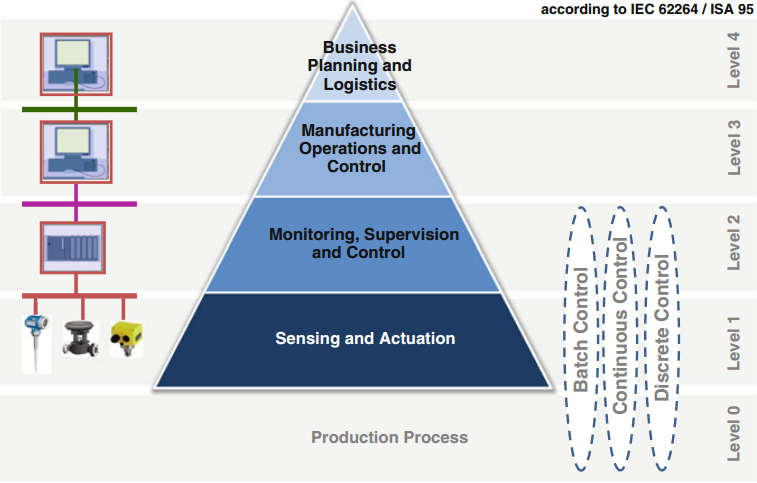
\includegraphics[scale=0.8]{Hierarquia.png}
  \label{fig:Hierarquia}
  \caption{Hierarquia funcional de acordo com a IEC 62264-3} \cite{colombo2014industrial}.
\end{figure}


No nível dois da hierarquia considerada, tem-se os Controladores Lógicos Programáveis (CLPs) que são utilizados como instrumentos intermediários entre os objetos físicos e o sistema SCADA. Esses controladores possuem design de entradas e saídas analógicas e digitais que podem interagir com  diversos objetos físicos de um sistema industrial (sensores e atuadores, por exemplo). Esses dispositivos são de essencial importância em sistemas industriais atuais devido a sua eficiência de captação de dados e facilidade de comunicação entre os níveis um e três da hierarquia funcional apresentada. Uma descrição mais detalhada acerca da utilização de sistemas SCADA e CLPs é apresentada ao decorrer desse trabalho. 

Sistemas de Supervisão e Aquisição de Dados (presentes no nível três da hierarquia descrita anteriormente) lidam com a obtenção de dados em tempo-real de locais remotos para controlar e monitorar algum processo, incluindo captação de dados e apresentação dos mesmos ao usuário. Esses sistemas são comumente utilizados em aplicações como usinas, refinarias de petróleo e gás, telecomunicações, transporte, controle de sistemas hídricos ou até mesmo em setores de assistência médica, como descrito em \cite{silva2015mobile}. Nesses últimos casos, sistemas SCADA disponibilizam soluções médicas e permitem profissionais da saúde monitorarem e controlarem o estado de saúde de um paciente de maneira eficiente e a custos cada vez mais baixos.

Tendo isso em vista, o Laboratório de Avaliação de Medição em Petróleo (LAMP), localizado na UFRN, vem modificando suas estruturas a fim de adequar suas instalações com os projetos que lá são executados. Em 2006, o o objetivo do laboratório era avaliar de forma automática as medições de vazão e BS\&W (Basic Sediments and Water) por meio de condições de simulação de operações de campo \cite{salazar2006instrumentaccao}. 

Atualmente, o LAMP continua desenvolvendo pesquisas na área de automação, instrumentação e eletrônica, tendo como principais atividades, projetos de simulação de sistemas petrolíferos, reaproveitando a instrumentação advinda dos projetos anteriores. Desse modo, é necessário o entendimento de instrumentos eletrônicos de controle e automação amplamente utilizados no setor industrial, tais quais CLPs, microcontroladores e sistemas supervisórios,  além de componentes básicos como sensores, válvulas e bombas a fim de dar continuidade aos projetos em desenvolvimento no laboratório.

\section{Objetivos}

Os principais objetivos desse trabalho são:

\begin{itemize}
\item Realizar a comunicação de elementos do sistema industrial atualmente presente no LAMP;
\item Desenvolver um protótipo de sistema supervisório que interaja com a planta industrial do laboratório de maneira satisfatória ao projeto que está sendo desenvolvido;
\item Identificar características, vantagens e desvantagens da utilização de diferentes equipamentos e tecnologias, tais quais descrições de diferentes controladores e formas de comunicação;
\item Documentar de maneira detalhada todo o processo realizado na comunicação e no desenvolvimento das atividades desse trabalho para que possam ser repetidas e implementadas futuramente por outras pessoas, de forma que seja possível adaptá-las a outros sistemas
\end{itemize}



\section{Estrutura do documento}
Este trabalho está estruturado em 5 capítulos. Nesse primeiro capítulo, foi realizada uma breve discussão sobre a evolução de sistemas industriais destacando a utilização de sistemas SCADA e CLPs. Além disso, foram apresentados os principais objetivos do trabalho. O capítulo 2 descreve a as instalações existentes no LAMP, considera especificações teóricas e técnicas e demonstra os instrumentos, softwares, protocolos e equipamentos utilizados nesse trabalho; o capítulo 3 apresenta as implementações feitas, descrevendo as configurações de cada elemento do sistema e explicando a comunicação entre eles; No capítulo 4, explica-se o desenvolvimento da aplicação utilizada e os testes desenvolvidos no sistema. Finalmente, o capítulo 5 apresenta conclusões, dificuldades encontradas e sugestões para trabalhos futuros.